\documentclass[15pt]{report}
\usepackage[utf8]{inputenc}
\usepackage[]{tikz}
\usepackage{amsmath}
\usepackage{animate}
\usepackage{fp}
\usepackage{graphicx}
\usepackage{pstricks}
\usepackage{media9}
\usepackage{xcolor}
\usepackage{pgfplots}
\usepackage{mathtools,amssymb}
\usepackage[x11names,table]{xcolor}

\begin{filecontents}{timeline.txt}
::0x0 % coordinate system & y=e^x, repeated until last frame
::1 % one blue curve per frame
::2
::3
::4
::5
::6
::7
::8
\end{filecontents}

\pgfplotsset{compat=1.7}

\usepackage[pagestyles]{titlesec}
\usepackage{titlesec} %para quitar chaptername
\titleformat{\chapter}[display]
  {\normalfont\bfseries}{}{0pt}{\Large}
    %

    %
\textheight = 23.5cm % largo texto impreso
\textwidth = 18cm % ancho texto impreso
\topmargin = -2cm % margen superior 3-2=1cm
\oddsidemargin = -1cm % margen izquierdo 4.5-2=2.5cm
% Sangría=0mm
\headheight = -0.5cm


%RENAME
\renewcommand{\chaptername}{\underline {Capítulo}}
\renewcommand{\contentsname}{CONTENIDO}
\renewcommand{\tablename}{Tabla}

\usepackage{etoolbox}
\makeatletter
\patchcmd{\chapter}{\if@openright\cleardoublepage\else\clearpage\fi}{}{}{}
\makeatother

\definecolor{usm}{RGB}{176,153,40}


\title{
        {\sc \bf \color{usm} PRUEBA DE HIPÓTESIS} 
        \\
        {\vfill}
        \\
        {
\includegraphics[scale=0.17]{unmsm1.png}}
        \\
        {}
        \\
        {Facultad de Ciencias Económicas}
       }
    \author{Rufasto C. Andy}
    \date{}
    

\begin{document}


\maketitle
\begingroup
\large
\tableofcontents
\endgroup
        \begingroup
        \large

\newpage
    \chapter{\color{usm}PASOS PARA LA PRUEBA DE HIPÓTESIS}
        	\begin{flushleft}
Prueba de Hipótesis sirve para validar aseveraciones sobre la población tomando como evidencia los datos de la muestra.
sean:\\
	
$\pmb{H_O}$: La hipótesis nula.\\
$\pmb{H_A}$: La hipótesis alternativa.\\
$\pmb{\theta}$ : Estimador.\\
$\pmb{\alpha}$: El nivel de significancia.\\

	\end{flushleft}
	\begin{enumerate}
\item	Se definen las hipótesis $H_0$ y $H_A$.\\
		donde $H_0$ asevera que no hay diferencias significativas en la población para poder aseverar $H_A$. Pueden hallarse tres 	diferentes casos:\\


\begin{enumerate}
\begin{minipage}[b]{\textwidth}
    \begin{minipage}[b]{0.3 \textwidth}\item
    	\begin{align*}
    	H_0&: \theta = \theta_0,\\
    	H_A&: \theta \neq \theta_0.
    	\end{align*}
        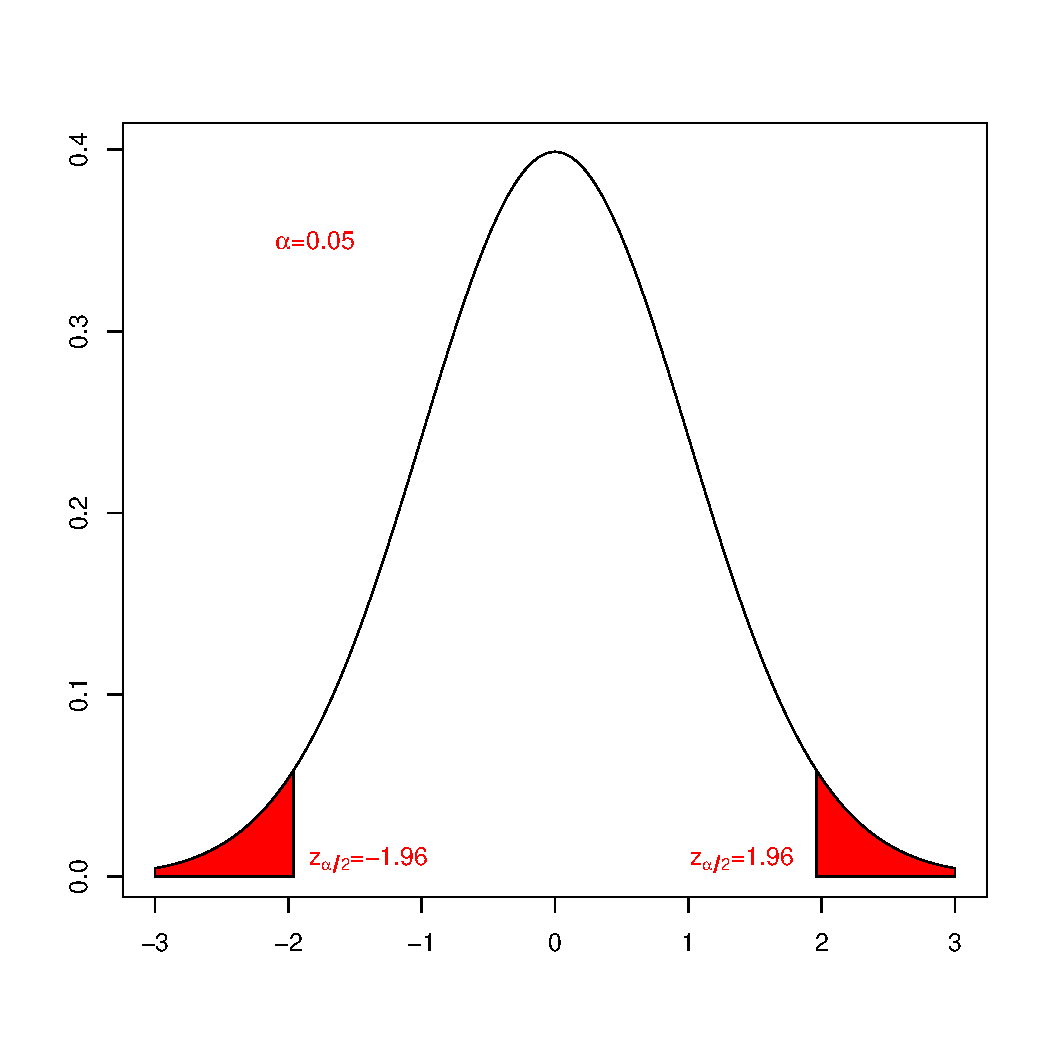
\includegraphics[height=5cm, width=6cm]{z05id.pdf}
    	\end{minipage} \hfill
    \begin{minipage}[b]{0.3 \textwidth}\item
		\begin{align*}
		H_0&: \theta \leq \theta_0,\\
    	H_A&: \theta > \theta_0. 
		\end{align*}
		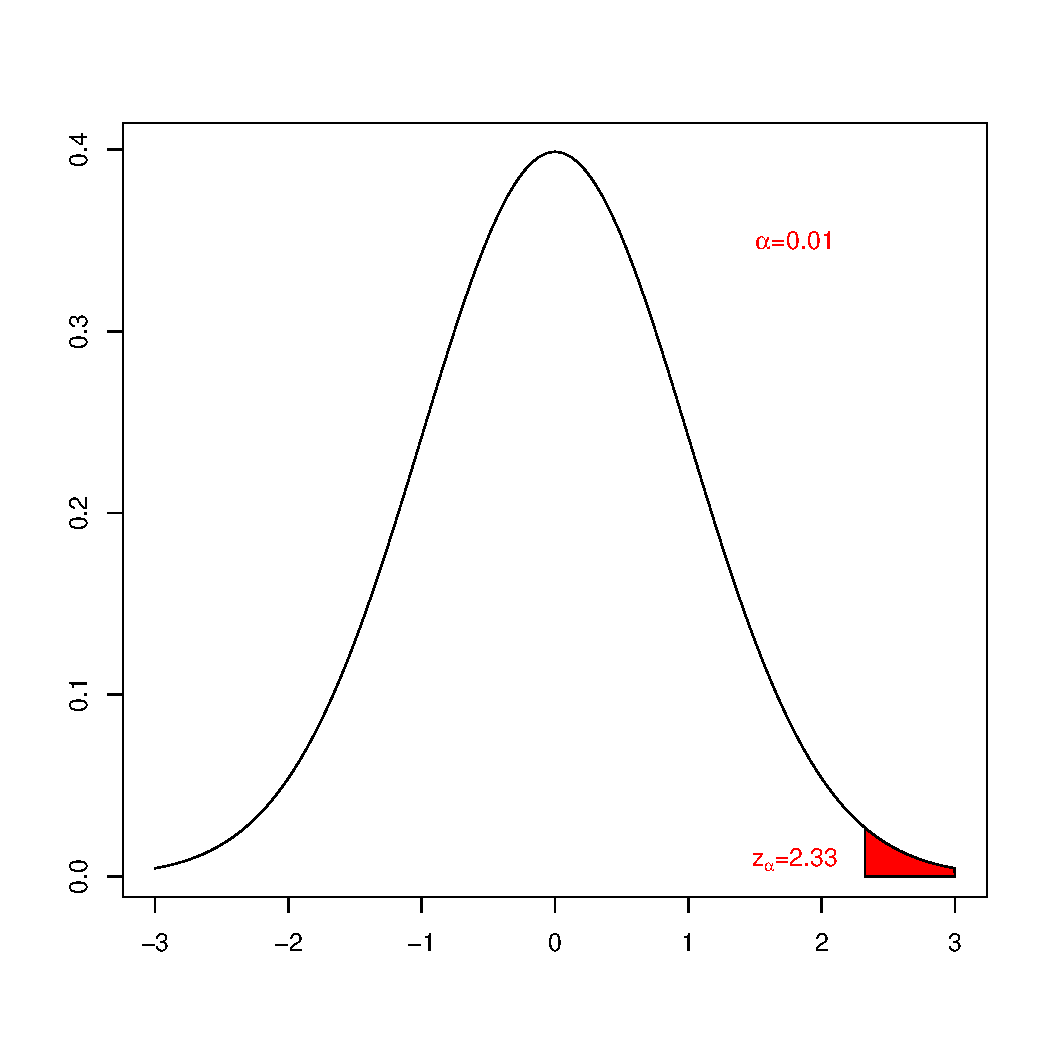
\includegraphics[height=5cm, width=6cm]{z01d.pdf}
		\end{minipage} \hfill
    \begin{minipage}[b]{0.3 \textwidth}\item
		\begin{align*}
		H_0&: \theta \geq \theta_0,\\
    	H_A&: \theta < \theta_0. 
		\end{align*}
		  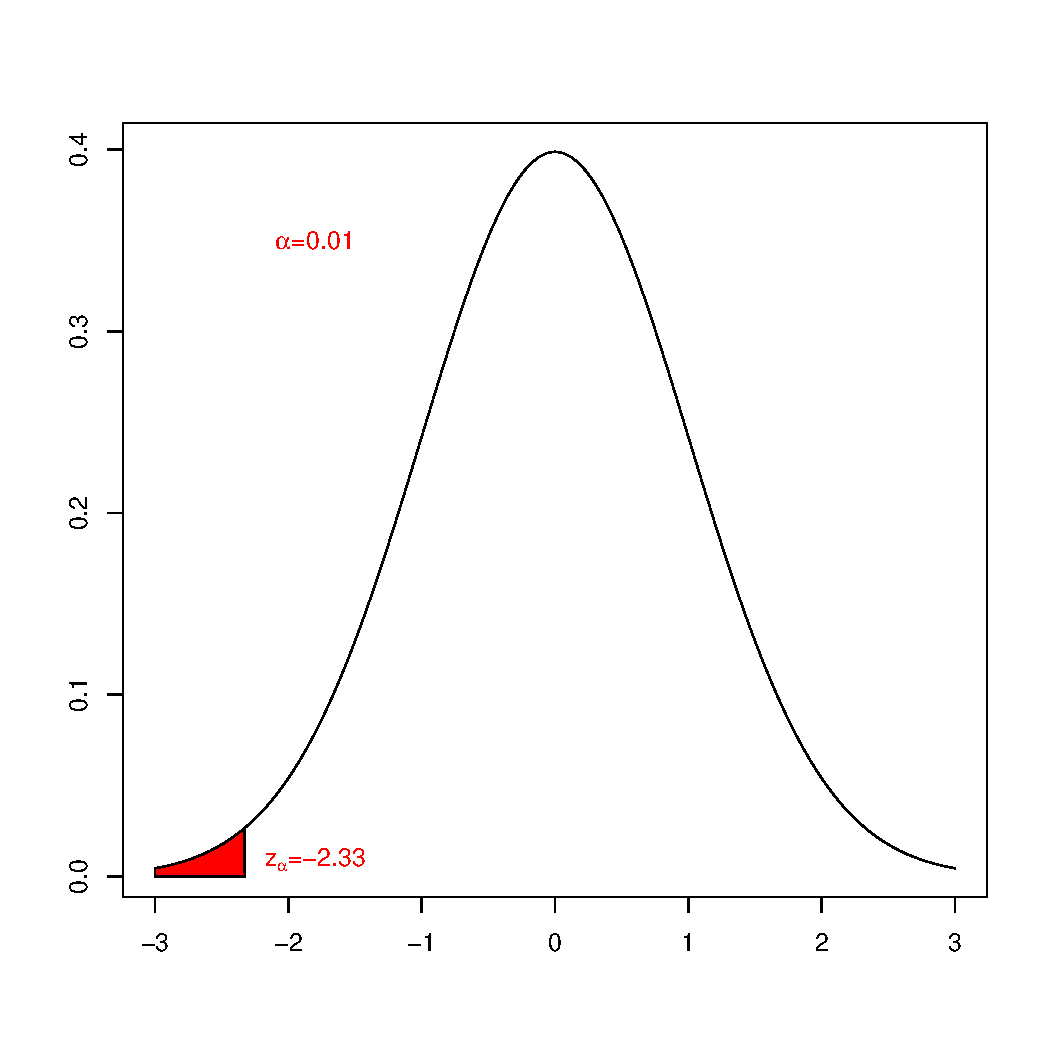
\includegraphics[height=5cm, width=6cm]{z01i.pdf}
    \end{minipage}
    \end{minipage}
\end{enumerate}
\item Se elige un nivel de significancia $\alpha$ que expresa el riesgo que se esta dispuesto a correr al hacer la investigación (error tipo I) Que representa la probabilidad de al aceptar $H_0$ ésta sea falsa.\\
El error tipo II es el  complemento de $\alpha$ ($1-\alpha$), representa la probabilidad de que al rechazar $H_0$ ésta sea verdadera.


\item Se identifica el tipo de distribución de probabilidad que sigue la muestra.
		
\item se identifica el estadístico de prueba.

\item Se establece la regla de decisión.

\item se toma la decisión.
		




	\end{enumerate}	

    \newpage
    \chapter{\color{usm}MEDIA POBLACIONAL}
    \section{Varianza Conocida}
        \begin{minipage}[c]{\textwidth}
    \begin{minipage}[c]{0.3 \textwidth}\item
    	\begin{align*}
    	H_0&: \mu = \mu_0,\\
    	H_A&: \mu \neq \mu_0.    	
    	\end{align*}\end{minipage} \hfill
    \begin{minipage}[b]{0.3 \textwidth}\item
				Rechazo	$H_0$ si:		
		\end{minipage} \hfill
    \begin{minipage}[c]{0.3 \textwidth}\item
	 $$\left|\frac { \bar{x}-\mu_0  }{ \sfrac { \sigma  }/{ \sqrt { n }  }  }\right|> Z_{\frac{\alpha}{2}}$$
    \end{minipage}
    \end{minipage}
    
    
	\begin{minipage}[c]{\textwidth}
    \begin{minipage}[c]{0.3 \textwidth}\item
    	\begin{align*}
    	H_0&: \mu \le \mu_0,\\
    	H_A&: \mu > \mu_0.    	
    	\end{align*}\end{minipage} \hfill
    \begin{minipage}[b]{0.3 \textwidth}\item
				Rechazo $H_0$ si:		
		\end{minipage} \hfill
    \begin{minipage}[c]{0.3 \textwidth}\item
	 $$\frac { \bar{x}-\mu_0  }{ \sfrac { \sigma  }/{ \sqrt { n }  }  }> Z_{\alpha}$$
    \end{minipage}
    \end{minipage}
    
		\begin{minipage}[b]{\textwidth}
    \begin{minipage}[c]{0.3 \textwidth}\item
    	\begin{align*}
    	H_0&: \mu \ge \mu_0,\\
    	H_A&: \mu < \mu_0.    	
    	\end{align*}\end{minipage} \hfill
    \begin{minipage}[c]{0.3 \textwidth}\item
				Rechazo $H_0$ si:		
		\end{minipage} \hfill
    \begin{minipage}[c]{0.3 \textwidth}\item
	 $$\frac { \bar{x}-\mu_0  }{ \sfrac { \sigma  }/{ \sqrt { n }  }  }< -Z_{\alpha}$$
    \end{minipage}
    \end{minipage}
    \section{Varianza Desconocida y $n<30$}
        

	\begin{minipage}[c]{\textwidth}
    \begin{minipage}[c]{0.3 \textwidth}\item
    	\begin{align*}
    	H_0&: \mu = \mu_0,\\
    	H_A&: \mu \neq \mu_0.    	
    	\end{align*}\end{minipage} \hfill
    \begin{minipage}[b]{0.3 \textwidth}\item
				Rechazo	$H_0$ si:		
		\end{minipage} \hfill
    \begin{minipage}[c]{0.3 \textwidth}\item
	 $$\left|\frac { \bar{x}-\mu_0  }{ \sfrac { s  }/{ \sqrt { n }  }  }\right| > t_{(n-1,\frac{\alpha}{2})}$$
    \end{minipage}
    \end{minipage}
    
    
	\begin{minipage}[c]{\textwidth}
    \begin{minipage}[c]{0.3 \textwidth}\item
    	\begin{align*}
    	H_0&: \mu \le \mu_0,\\
    	H_A&: \mu > \mu_0.    	
    	\end{align*}\end{minipage} \hfill
    \begin{minipage}[b]{0.3 \textwidth}\item
				Rechazo $H_0$ si:		
		\end{minipage} \hfill
    \begin{minipage}[c]{0.3 \textwidth}\item
	 $$\frac { \bar{x}-\mu_0  }{ \sfrac { s  }/{ \sqrt { n }  }  }> t_{(n-1,\alpha)}$$
    \end{minipage}
    \end{minipage}
    
		\begin{minipage}[b]{\textwidth}
    \begin{minipage}[c]{0.3 \textwidth}\item
    	\begin{align*}
    	H_0&: \mu \ge \mu_0,\\
    	H_A&: \mu < \mu_0.    	
    	\end{align*}\end{minipage} \hfill
    \begin{minipage}[c]{0.3 \textwidth}\item
				Rechazo $H_0$ si:		
		\end{minipage} \hfill
    \begin{minipage}[c]{0.3 \textwidth}\item
	 $$\frac { \bar{x}-\mu_0  }{ \sfrac {  s }/{ \sqrt { n }  }  }<- t_{(n-1,\alpha)}$$
    \end{minipage}
    \end{minipage}
        \newpage
     \chapter{\color{usm}PROPORCION POBLACIONAL}
        
	\begin{minipage}[c]{\textwidth}
    \begin{minipage}[c]{0.3 \textwidth}\item
    	\begin{align*}
    	H_0&: P = P_0,\\
    	H_A&: P \neq P_0.    	
    	\end{align*}\end{minipage} \hfill
    \begin{minipage}[b]{0.3 \textwidth}\item
				Rechazo	$H_0$ si:		
		\end{minipage} \hfill
    \begin{minipage}[c]{0.3 \textwidth}\item
	 $$\left|\frac { p-P_{ 0 } }{ \sqrt { \frac { p_{ 0 }q_{ 0 } }{ n }  }  } \right| > Z_{\frac{\alpha}{2}}$$
    \end{minipage}
    \end{minipage}
    
    
	\begin{minipage}[c]{\textwidth}
    \begin{minipage}[c]{0.3 \textwidth}\item
    	\begin{align*}
    	H_0&: P \le P_0,\\
    	H_A&: P > P_0.    	
    	\end{align*}\end{minipage} \hfill
    \begin{minipage}[b]{0.3 \textwidth}\item
				Rechazo $H_0$ si:		
		\end{minipage} \hfill
    \begin{minipage}[c]{0.3 \textwidth}\item
	 $$\frac { p-P_{ 0 } }{ \sqrt { \frac { p_{ 0 }q_{ 0 } }{ n }  }  } > Z_{\alpha}$$
    \end{minipage}
    \end{minipage}
    
		\begin{minipage}[b]{\textwidth}
    \begin{minipage}[c]{0.3 \textwidth}\item
    	\begin{align*}
    	H_0&: P \ge P_0,\\
    	H_A&: P < P_0.    	
    	\end{align*}\end{minipage} \hfill
    \begin{minipage}[c]{0.3 \textwidth}\item
				Rechazo $H_0$ si:		
		\end{minipage} \hfill
    \begin{minipage}[c]{0.3 \textwidth}\item
	 $$\frac { p-P_{ 0 } }{ \sqrt { \frac { p_{ 0 }q_{ 0 } }{ n }  }  } <- Z_{\alpha}$$
    \end{minipage}
    \end{minipage} 

     
     \chapter{\color{usm}VARIANZA POBLACIONAL}
          
	\begin{minipage}[c]{\textwidth}
    \begin{minipage}[c]{0.3 \textwidth}\item
    	\begin{align*}
    	H_0&: \sigma^{2} = \sigma^{2}_0,\\
    	H_A&: \sigma^{2} \neq \sigma^{2}_0.    	
    	\end{align*}\end{minipage} \hfill
    \begin{minipage}[b]{0.3 \textwidth}\item
				Rechazo	$H_0$ si:		
		\end{minipage} \hfill
    \begin{minipage}[c]{0.3 \textwidth}\item
	 $$\frac { (n-1)s^{ 2 } }{ \sigma ^{ 2 }_{ 0 } }\notin \left( \chi ^{ 2 }_{ \frac { \alpha  }{ 2 }  };\chi ^{ 2 }_{ 1-\frac { \alpha  }{ 2 }  } \right)  $$
    \end{minipage}
    \end{minipage}
    
    
	\begin{minipage}[c]{\textwidth}
    \begin{minipage}[c]{0.3 \textwidth}\item
    	\begin{align*}
    	H_0&: \sigma^{2} \le \sigma^{2}_0,\\
    	H_A&: \sigma^{2} > \sigma^{2}_0.    	
    	\end{align*}\end{minipage} \hfill
    \begin{minipage}[b]{0.3 \textwidth}\item
				Rechazo $H_0$ si:		
		\end{minipage} \hfill
    \begin{minipage}[c]{0.3 \textwidth}\item
	 $$\frac { (n-1)s^{ 2 } }{ \sigma ^{ 2 }_{ 0 } } }>\chi^2_{\alpha}$$
    \end{minipage}
    \end{minipage}
    
		\begin{minipage}[b]{\textwidth}
    \begin{minipage}[c]{0.3 \textwidth}\item
    	\begin{align*}
    	H_0&: \sigma^{2} \ge \sigma^{2}_0,\\
    	H_A&: \sigma^{2} < \sigma^{2}_0.    	
    	\end{align*}\end{minipage} \hfill
    \begin{minipage}[c]{0.3 \textwidth}\item
				Rechazo $H_0$ si:		
		\end{minipage} \hfill
    \begin{minipage}[c]{0.3 \textwidth}\item
	 $$\frac { (n-1)s^{ 2 } }{ \sigma ^{ 2 }_{ 0 } } }<\chi^2_{1-\alpha}$$
    \end{minipage}
    \end{minipage}
        \newpage
    \chapter{\color{usm} DIFERENCIAS POBLACIONALES}
        \section{Varianzas Conocidas}
            
\begin{minipage}[c]{\textwidth}
    \begin{minipage}[c]{0.3 \textwidth}\item
    	\begin{align*}
    	H_0&: \mu _{ \bar { x } _{ 1 }-\bar { x } _{ 2 }} = \mu _{ \bar { x } _{ 1 }-\bar { x } _{ 2 }}_0,\\
    	H_A&: \mu _{ \bar { x } _{ 1 }-\bar { x } _{ 2 }} \neq \mu _{ \bar { x } _{ 1 }-\bar { x } _{ 2 }}_0.    	
    	\end{align*}\end{minipage} \hfill
    \begin{minipage}[b]{0.3 \textwidth}\item
				Rechazo	$H_0$ si:		
		\end{minipage} \hfill
    \begin{minipage}[c]{0.3 \textwidth}\item
	 $$\left|\frac {( \bar{x}_1-\bar{x}_2)-(\mu _{ \bar { x } _{ 1 }-\bar { x } _{ 2 }}_0 )}{\sqrt{\frac { \sigma^ 2_1 }{n_1} +\frac { \sigma^ 2_2 }{n_2}}  }\right|> Z_{\frac{\alpha}{2}}$$
    \end{minipage}
    \end{minipage}
    
    
	\begin{minipage}[c]{\textwidth}
    \begin{minipage}[c]{0.3 \textwidth}\item
    	\begin{align*}
    	H_0&: \mu _{ \bar { x } _{ 1 }-\bar { x } _{ 2 }} \le \mu _{ \bar { x } _{ 1 }-\bar { x } _{ 2 }}_0,\\
    	H_A&: \mu _{ \bar { x } _{ 1 }-\bar { x } _{ 2 }} > \mu _{ \bar { x } _{ 1 }-\bar { x } _{ 2 }}_0.    	
    	\end{align*}\end{minipage} \hfill
    \begin{minipage}[b]{0.3 \textwidth}\item
				Rechazo $H_0$ si:		
		\end{minipage} \hfill
    \begin{minipage}[c]{0.3 \textwidth}\item
	 $$\frac {( \bar{x}_1-\bar{x}_2)-(\mu _{ \bar { x } _{ 1 }-\bar { x } _{ 2 }}_0 )}{\sqrt{\frac { \sigma^ 2_1 }{n_1} +\frac { \sigma^ 2_2 }{n_2}}  }> Z_{\alpha}$$
    \end{minipage}
    \end{minipage}
    
		\begin{minipage}[b]{\textwidth}
    \begin{minipage}[c]{0.3 \textwidth}\item
    	\begin{align*}
    	H_0&: \mu _{ \bar { x } _{ 1 }-\bar { x } _{ 2 }} \ge \mu _{ \bar { x } _{ 1 }-\bar { x } _{ 2 }}_0,\\
    	H_A&: \mu _{ \bar { x } _{ 1 }-\bar { x } _{ 2 }} < \mu _{ \bar { x } _{ 1 }-\bar { x } _{ 2 }}_0.    	
    	\end{align*}\end{minipage} \hfill
    \begin{minipage}[c]{0.3 \textwidth}\item
				Rechazo $H_0$ si:		
		\end{minipage} \hfill
    \begin{minipage}[c]{0.3 \textwidth}\item
	 $$\frac {( \bar{x}_1-\bar{x}_2)-(\mu _{ \bar { x } _{ 1 }-\bar { x } _{ 2 }}_0 )}{\sqrt{\frac { \sigma^ 2_1 }{n_1} +\frac { \sigma^ 2_2 }{n_2}}  }< -Z_{\alpha}$$
    \end{minipage}
    \end{minipage}
        \section{Varianzas Desconocidas e iguales}
                

\begin{minipage}[c]{\textwidth}
    \begin{minipage}[c]{0.3 \textwidth}\item
    	\begin{align*}
    	H_0&: \mu _{ \bar { x } _{ 1 }-\bar { x } _{ 2 }} = \mu _{ \bar { x } _{ 1 }-\bar { x } _{ 2 }}_0,\\
    	H_A&: \mu _{ \bar { x } _{ 1 }-\bar { x } _{ 2 }} \neq \mu _{ \bar { x } _{ 1 }-\bar { x } _{ 2 }}_0.    	
    	\end{align*}\end{minipage} \hfill
    \begin{minipage}[b]{0.3 \textwidth}\item
				Rechazo	$H_0$ si:		
		\end{minipage} \hfill
    \begin{minipage}[c]{0.3 \textwidth}\item
	 $$\left|\frac { (\bar { x } _{ 1 }-\bar { x } _{ 2 })-(\mu _{ \bar { x } _{ 1 }-\bar { x } _{ 2 } }_{ 0 }) }{ \sqrt { \frac { (n_{ 1 }-1)s^{ 2 }_{ 1 }+(n_{ 2 }-1)s^{ 2 }_{ 2 } }{ n_{ 1 }-n_{ 2 }-2 }   \left( \frac { 1 }{ n_{ 1 } } +\frac { 1 }{ n_{ 2 } }  \right)  } }\right|> Z_{\frac{\alpha}{2}}$$
    \end{minipage}
    \end{minipage}
    
    
	\begin{minipage}[c]{\textwidth}
    \begin{minipage}[c]{0.3 \textwidth}\item
    	\begin{align*}
    	H_0&: \mu _{ \bar { x } _{ 1 }-\bar { x } _{ 2 }} \le \mu _{ \bar { x } _{ 1 }-\bar { x } _{ 2 }}_0,\\
    	H_A&: \mu _{ \bar { x } _{ 1 }-\bar { x } _{ 2 }} > \mu _{ \bar { x } _{ 1 }-\bar { x } _{ 2 }}_0.    	
    	\end{align*}\end{minipage} \hfill
    \begin{minipage}[b]{0.3 \textwidth}\item
				Rechazo $H_0$ si:		
		\end{minipage} \hfill
    \begin{minipage}[c]{0.3 \textwidth}\item
	 $$\frac { (\bar { x } _{ 1 }-\bar { x } _{ 2 })-(\mu _{ \bar { x } _{ 1 }-\bar { x } _{ 2 } }_{ 0 }) }{ \sqrt { \frac { (n_{ 1 }-1)s^{ 2 }_{ 1 }+(n_{ 2 }-1)s^{ 2 }_{ 2 } }{ n_{ 1 }-n_{ 2 }-2 }   \left( \frac { 1 }{ n_{ 1 } } +\frac { 1 }{ n_{ 2 } }  \right)  } }> Z_{\alpha}$$
    \end{minipage}
    \end{minipage}
    
		\begin{minipage}[b]{\textwidth}
    \begin{minipage}[c]{0.3 \textwidth}\item
    	\begin{align*}
    	H_0&: \mu _{ \bar { x } _{ 1 }-\bar { x } _{ 2 }} \ge \mu _{ \bar { x } _{ 1 }-\bar { x } _{ 2 }}_0,\\
    	H_A&: \mu _{ \bar { x } _{ 1 }-\bar { x } _{ 2 }} < \mu _{ \bar { x } _{ 1 }-\bar { x } _{ 2 }}_0.    	
    	\end{align*}\end{minipage} \hfill
    \begin{minipage}[c]{0.3 \textwidth}\item
				Rechazo $H_0$ si:		
		\end{minipage} \hfill
    \begin{minipage}[c]{0.3 \textwidth}\item
	 $$\frac { (\bar { x } _{ 1 }-\bar { x } _{ 2 })-(\mu _{ \bar { x } _{ 1 }-\bar { x } _{ 2 } }_{ 0 }) }{ \sqrt { \frac { (n_{ 1 }-1)s^{ 2 }_{ 1 }+(n_{ 2 }-1)s^{ 2 }_{ 2 } }{ n_{ 1 }-n_{ 2 }-2 }   \left( \frac { 1 }{ n_{ 1 } } +\frac { 1 }{ n_{ 2 } }  \right)  } }< -Z_{\alpha}$$
    \end{minipage}
    \end{minipage}

            \newpage
        \section{Varianzas Desconocidas y diferentes}
            
\begin{minipage}[c]{\textwidth}
    \begin{minipage}[c]{0.3 \textwidth}\item
    	\begin{align*}
    	H_0&: \mu _{ \bar { x } _{ 1 }-\bar { x } _{ 2 }} = \mu _{ \bar { x } _{ 1 }-\bar { x } _{ 2 }}_0,\\
    	H_A&: \mu _{ \bar { x } _{ 1 }-\bar { x } _{ 2 }} \neq \mu _{ \bar { x } _{ 1 }-\bar { x } _{ 2 }}_0.    	
    	\end{align*}\end{minipage} \hfill
    \begin{minipage}[b]{0.3 \textwidth}\item
				Rechazo	$H_0$ si:		
		\end{minipage} \hfill
    \begin{minipage}[c]{0.3 \textwidth}\item
	 $$\left|\frac {( \bar{x}_1-\bar{x}_2)-(\mu _{ \bar { x } _{ 1 }-\bar { x } _{ 2 }}_0 )}{\sqrt{\frac { \sigma^ 2_1 }{n_1} +\frac { \sigma^ 2_2 }{n_2}}  }\right|> t_{(v,\frac{\alpha}{2})}$$
    \end{minipage}
    \end{minipage}
    
    
	\begin{minipage}[c]{\textwidth}
    \begin{minipage}[c]{0.3 \textwidth}\item
    	\begin{align*}
    	H_0&: \mu _{ \bar { x } _{ 1 }-\bar { x } _{ 2 }} \le \mu _{ \bar { x } _{ 1 }-\bar { x } _{ 2 }}_0,\\
    	H_A&: \mu _{ \bar { x } _{ 1 }-\bar { x } _{ 2 }} > \mu _{ \bar { x } _{ 1 }-\bar { x } _{ 2 }}_0.    	
    	\end{align*}\end{minipage} \hfill
    \begin{minipage}[b]{0.3 \textwidth}\item
				Rechazo $H_0$ si:		
		\end{minipage} \hfill
    \begin{minipage}[c]{0.3 \textwidth}\item
	 $$\frac {( \bar{x}_1-\bar{x}_2)-(\mu _{ \bar { x } _{ 1 }-\bar { x } _{ 2 }}_0 )}{\sqrt{\frac { \sigma^ 2_1 }{n_1} +\frac { \sigma^ 2_2 }{n_2}}  }> t_{(v,\alpha)}$$
    \end{minipage}
    \end{minipage}
    
		\begin{minipage}[b]{\textwidth}
    \begin{minipage}[c]{0.3 \textwidth}\item
    	\begin{align*}
    	H_0&: \mu _{ \bar { x } _{ 1 }-\bar { x } _{ 2 }} \ge \mu _{ \bar { x } _{ 1 }-\bar { x } _{ 2 }}_0,\\
    	H_A&: \mu _{ \bar { x } _{ 1 }-\bar { x } _{ 2 }} < \mu _{ \bar { x } _{ 1 }-\bar { x } _{ 2 }}_0.    	
    	\end{align*}\end{minipage} \hfill
    \begin{minipage}[c]{0.3 \textwidth}\item
				Rechazo $H_0$ si:		
		\end{minipage} \hfill
    \begin{minipage}[c]{0.3 \textwidth}\item
	 $$\frac {( \bar{x}_1-\bar{x}_2)-(\mu _{ \bar { x } _{ 1 }-\bar { x } _{ 2 }}_0 )}{\sqrt{\frac { \sigma^ 2_1 }{n_1} +\frac { \sigma^ 2_2 }{n_2}}  }< -t_{(v,\alpha)}$$
    \end{minipage}
    \end{minipage}
    
$$
v\approx \left\{ \frac { \left( \frac { s^{ 2 }_{ 1 } }{ n_{ 1 } } +\frac { s^{ 2 }_{ 2 } }{ n_{ 2 } }  \right) ^{ 2 } }{ \frac { \left( \frac { s^{ 2 }_{ 1 } }{ n_{ 1 } }  \right) ^{ 2 } }{ n_{ 1 }-1 } +\frac { \left( \frac { s^{ 2 }_{ 2 } }{ n_{ 2 } }  \right) ^{ 2 } }{ n_{ 2 }-1 }  }  \right\} 

$$  
    \chapter{\color{usm}DIFERENCIA DE PROPORCIONES}
            \begin{minipage}[c]{\textwidth}
    \begin{minipage}[c]{0.3 \textwidth}\item
    	\begin{align*}
    	H_0&: (P_{1}-P_{2}) = (P_{1}-P_{2})_0,\\
    	H_A&: (P_{1}-P_{2}) = (P_{1}-P_{2})_0.    	
    	\end{align*}\end{minipage} \hfill
    \begin{minipage}[b]{0.3 \textwidth}\item
				Rechazo	$H_0$ si:		
		\end{minipage} \hfill
    \begin{minipage}[c]{0.3 \textwidth}\item
	 $$\left|\frac { (p_{ 1 }-p_{ 2 })-(P_{ 1 }-P_{ 2 }) }{ \sqrt { \frac { p_{ 1 }q_{ 1 } }{ n_{ 1 } } +\frac { p_{ 2 }q_{ 2 } }{ n_{ 2 } }  }  }  \right| > Z_{\frac{\alpha}{2}}$$
    \end{minipage}
    \end{minipage}
    
    
	\begin{minipage}[c]{\textwidth}
    \begin{minipage}[c]{0.3 \textwidth}\item
    	\begin{align*}
    	H_0&: (P_{1}-P_{2}) \le (P_{1}-P_{2})_0,\\
    	H_A&: (P_{1}-P_{2}) > (P_{1}-P_{2})_0.    	
    	\end{align*}\end{minipage} \hfill
    \begin{minipage}[b]{0.3 \textwidth}\item
				Rechazo $H_0$ si:		
		\end{minipage} \hfill
    \begin{minipage}[c]{0.3 \textwidth}\item
	 $$\frac { (p_{ 1 }-p_{ 2 })-(P_{ 1 }-P_{ 2 }) }{ \sqrt { \frac { p_{ 1 }q_{ 1 } }{ n_{ 1 } } +\frac { p_{ 2 }q_{ 2 } }{ n_{ 2 } }  }  }  > Z_{\alpha}$$
    \end{minipage}
    \end{minipage}
    
		\begin{minipage}[b]{\textwidth}
    \begin{minipage}[c]{0.3 \textwidth}\item
    	\begin{align*}
    	H_0&: (P_{1}-P_{2}) \ge (P_{1}-P_{2})_0,\\
    	H_A&: (P_{1}-P_{2}) < (P_{1}-P_{2})_0.    	
    	\end{align*}\end{minipage} \hfill
    \begin{minipage}[c]{0.3 \textwidth}\item
				Rechazo $H_0$ si:		
		\end{minipage} \hfill
    \begin{minipage}[c]{0.3 \textwidth}\item
	 $$\frac { (p_{ 1 }-p_{ 2 })-(P_{ 1 }-P_{ 2 }) }{ \sqrt { \frac { p_{ 1 }q_{ 1 } }{ n_{ 1 } } +\frac { p_{ 2 }q_{ 2 } }{ n_{ 2 } }  }  }  <- Z_{\alpha}$$
    \end{minipage}
    \end{minipage} 
            \newpage
    \chapter{\color{usm}ANOVA}
            $
H_0: \mu_1=\mu_2=\hdots \mu_k=\mu_0 \\
$
$
H_A:\quad \exists\quad i\quad / \quad \mu_i \neq \mu_0
$

\begin{align*}
F_0  =& \quad \frac{Variabilidad \quad entre \quad grupos}{Variabilidad \quad intra \quad grupos}\\
    =& \quad \frac{CM_{entre} }{CM_{intra}}\\
\end{align*}
\begin{minipage}[b]{\textwidth}
    \begin{minipage}[b]{0.5 \textwidth}
\begin{align*}
CM_{entre}=&\quad\frac{SC_{entre}}{gl_{entre}}\\
=&\quad n_i\sum(\bar{X_i}-\bar{\bar{X}})^2\\
=&\quad \sum \frac{T^2_i}{n_i}-\frac{G^2}{N}
\end{align*}    

    \end{minipage} \hfill
    \begin{minipage}[b]{0.5 \textwidth}
\begin{align*}
CM_{intra}=&\quad\frac{SC_{intra}}{gl_{intra}}\\
=&\quad \sum(\bar{X_{ij}}-\bar{X})^2\\
=&\quad \sum X^2_{ij}-\sum \frac{T^2_i}{n_i}
\end{align*}    
    \end{minipage}
    \end{minipage}
    
    

          \begin{table}[h!]
         \centering
         \begin{tabular}{|l|c|c|c|c|} \hline
             Factor de Variación & SC & gl & CM & $F_0$\\ \hline
             Entre los grupos & $SC_{entre}$ &k-1&$\frac{SC_{entre}}{k-1}$ &\\
             Dentro de los grupos & $SC_{intra}$ &n-k&$\frac{SC_{intra}}{n-kk}$ & \\ \hline
             Total & $SC_{Total}$& & & \\ \hline
             
         \end{tabular}
         \caption{Tabla de Análisis de Varianza}
         \label{tab:my_label}
     \end{table}


Rechazo $H_0$ si $F_{(1-\alpha; k-1; n-k)} < F_0$

        \endgroup
\end{document}
